\section{Leitungen}

\subsection{Leitungsparameter}

\subsubsection{Doppelleitung:}
\[
    a = \text{Leiter Radius} \qquad d = \text{Abstand zw. den Leitern} \\
\]

\begin{tikzpicture}
    \tikzset{cross/.style={cross out, draw=black, minimum size=2*(#1-\pgflinewidth), inner sep=0pt, outer sep=0pt},
        %     %default radius will be 1pt. 
        cross/.default={3.5pt}}

        %linker Außenleiter
        \draw[-](-0.53,0.53)--(0.97,2.03);

        
        \draw[-](48:0.75) arc (48:312:0.75);

        %linker Innenleiter
        \draw[dashed](-0.106,0.106)--(0.41,0.622);
        \draw[dashed](0.106,-0.106)--(0.922,0.71);

        \draw[-](0,0) circle (0.15);
        \draw(0,0) node [cross] {};


        
        %%%%%%%%%%%%%%%%%%%%%%%%%%%%%%%%%%%%%%%%%%%%%%%%%%%%%%%%%%%
        %%%%%%%%%%%%%%%%%%%%%%%%%%%%%%%%%%%%%%%%%%%%%%%%%%%%%%%%%%%

        %Rechter Außenleiter
        \draw[-](0.48,0.58)--(1.97,2.03);
        \draw[-](1.53,-0.53)--(2.63,0.57);

        %Rechter Innenleiter
        \draw[dashed](0.894,0.106)--(1.41,0.622);
        \draw[dashed](1.106,-0.106)--(1.622,0.41);

        \draw[-](1,0) circle (0.15);
        \draw[-,fill=black!100] (1,0) circle (0.05);

        \draw([shift={(228:0.75)}]1,0) arc (-132:132:0.75);

\end{tikzpicture}

{\renewcommand*{\arraystretch}{0.2}
    \begin{tabularx}{0.5\columnwidth}{|X|}
        \hline
        \[R  = \frac{1}{\pi a\delta\sigma_c}\]              \\
        \hline
        \[L = \frac{\mu}{\pi} \cosh^{-1}\frac{d}{2a}\]      \\
        \hline
        \[G = \frac{\pi\sigma}{\cosh^{-1}(^d/_{2a})}\]      \\
        \hline
        \[C = \frac{\pi\varepsilon}{\cosh^{-1}(^d/_{2a})}\] \\
        \hline
    \end{tabularx}}

\subsubsection{Koaxial Leitung}
\[
    a = \text{innen Radius} \qquad b = \text{außen Radius} \\
\]
\begin{align*}
    \vec{H}(r, z) & = \frac{I}{2\pi r}\cdot e^{-j\beta z}\cdot\vec{e}_\varphi                    \\
    \vec{E}(r, z) & = \frac{I}{2\pi r}\cdot Z_F\cdot e^{-j\beta z} \cdot\vec{e}_r                \\
                  & = \frac{\hat{U}}{r \cdot\ln{(^{2b}/_{2a})}}\cdot e^{-j\beta z}\cdot\vec{e}_r
\end{align*}

\begin{tikzpicture}
    \tikzset{cross/.style={cross out, draw=black, minimum size=2*(#1-\pgflinewidth), inner sep=0pt, outer sep=0pt},
        %     %default radius will be 1pt. 
        cross/.default={3.5pt}}

        %Außenleiter
        \draw[-](-0.53,0.53)--(0.97,2.03);
        \draw[-](0.53,-0.53)--(1.63,0.57);

        \draw[-](0,0) circle (0.75);

        %Innenleiter
        \draw[-](-0.106,0.106)--(0.41,0.622);
        \draw[-](0.106,-0.106)--(0.622,0.41);

        \draw[-](0,0) circle (0.15);
        \draw(0,0) node [cross] {};

\end{tikzpicture}
{\renewcommand*{\arraystretch}{0.2}
    \begin{tabularx}{0.5\columnwidth}{|X|}
        \hline
        \[R=\frac{1}{2\pi\delta\sigma_c}\left[\frac{1}{a}+\frac{1}{b}\right]\] \\
        \hline
        \[L=\frac{\mu}{2\pi}\ln\frac{b}{a}\]                                   \\
        \hline
        \[G=\frac{2\pi\sigma}{\ln(^b/_a)}\]                                    \\
        \hline
        \[C=\frac{2\pi\varepsilon}{\ln(^b/_a)}\]                               \\
        \hline
    \end{tabularx}}

\subsubsection{Parallele Platten}
\[
    w  = \text{Platten Breite} \qquad d  = \text{Abstand zw. Platten}
\]

\begin{tikzpicture}
    \tikzset{cross/.style={cross out, draw=black, minimum size=2*(#1-\pgflinewidth), inner sep=0pt, outer sep=0pt},
        %     %default radius will be 1pt. 
        cross/.default={3.5pt}}

        %Untereplatte
        \draw[-](0,0)--(0,0.35);
        \draw[-](2,0)--(2,0.35);

        \draw[-](0,0)--(2,0);
        \draw[-](0,0.35)--(2,0.35);

        \draw[-](0,0.35)--(0.3,0.65);
        \draw[-](2,0)--(2.75,0.75);
        \draw[-](2,0.35)--(2.75,1.15);

        \draw[-](1,0.175) circle (0.15);
        \draw[-,fill=black!100] (1,0.175) circle (0.05);

        %Obere Platte
        \draw[-](0,0.65)--(0,1);
        \draw[-](2,0.65)--(2,1);

        \draw[-](0,0.65)--(2,0.65);
        \draw[-](0,1)--(2,1);

        \draw[-](0,1)--(0.75,1.75);
        \draw[-](2,1)--(2.75,1.75);
        \draw[-](2,0.65)--(2.75,1.4);

        \draw[-](1,0.825) circle (0.15);
        \draw(1,0.825) node [cross] {};
   
\end{tikzpicture}

{\renewcommand*{\arraystretch}{0.2}
    \begin{tabularx}{0.5\columnwidth}{|X|}
        \hline
        \[R=\frac{2}{w\delta\sigma}\] \\
        \hline
        \[L=\frac{\mu d}{w}\]         \\
        \hline
        \[G=\frac{\sigma w}{d}\]      \\
        \hline
        \[C=\frac{w\varepsilon}{d}\]  \\
        \hline
    \end{tabularx}}

\vspace{1ex}
Für beliebige Leitergeometrie gelten folgende Zusammenhänge:
\[
    LC = \mu\varepsilon \quad \text{und} \quad \frac{G}{C} = \frac{\sigma}{\varepsilon}
\]

\subsection{Allgemeine Lösung Leitungsgleichung}
\begin{align*}
    U(z) & = U^+ e^{\gamma z} + U^- e^{-\gamma z} = U^+ e^{\gamma d} + U^ - e^{-\gamma d}                      \\
    I(z) & = I^+ e^{\gamma z} + I^- e^{-\gamma z} = \frac{U^+}{Z_L}e^{\gamma d} - \frac{U^-}{Z_L}e^{-\gamma d} \\
    Z_L  & = \frac{U^+}{I^+} = \sqrt{ \frac{R + j \omega L}{G + j \omega C}}
\end{align*}

\begin{align*}
    \gamma      & = j \omega \sqrt{LC} \cdot \sqrt{ \frac{RG}{j^2 \omega^2 LC} + \frac{G}{j \omega C} + \frac{R}{j \omega L} + 1}                             \\
    \lambda     & = \frac{2 \pi}{\beta}                                                                                                                       \\
    v_{Ph}      & = \frac{\omega}{\beta}                                                                                                                      \\
    l_{elektr.} & = \beta \cdot l                                                                                                                             \\
    \alpha      & = \omega \cdot \sqrt{\dfrac{\mu \varepsilon}{2}\cdot \left(\sqrt{1+\dfrac{\sigma^2}{\omega^2\cdot\varepsilon^2}}{\color{red}{-}}1\right)}   \\
    \beta       & = \omega \cdot \sqrt{\dfrac{\mu \varepsilon}{2}\cdot \left(\sqrt{1+\dfrac{\sigma^2}{\omega^2\cdot\varepsilon^2}}{\color{green}{+}}1\right)}
\end{align*}

\subsubsection{Verlustlose Übertragungsleitung}
\begin{align*}
    \underline{\gamma} & = j\omega\sqrt{LC}= j\beta                                                                                           \\
    Z_L                & =\frac{U^+}{U^-}       = \sqrt{\frac{L}{C}}                                                                          \\
    v                  & = \frac{\omega}{\beta} = \frac{1}{\sqrt{LC}}= \frac{1}{\sqrt{\mu\varepsilon}}= \frac{c_0}{\sqrt{\mu_r\varepsilon_r}} \\
    \lambda            & = \frac{2\pi}{\beta}=\frac{1}{f\sqrt{LC}}= \frac{v}{f}= \frac{c_0}{f\sqrt{\mu_r\varepsilon_r}}
\end{align*}

\subsubsection{vernachlässigbarer Widerstandsbelag}
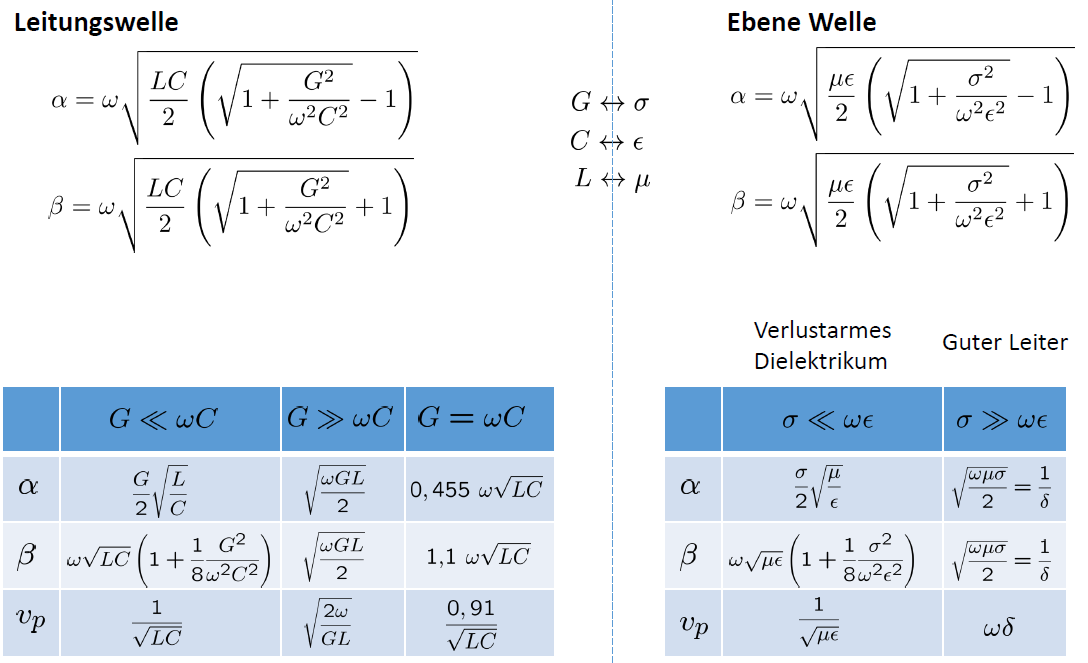
\includegraphics[width=\columnwidth]{Figures/vernachlaessigbarerWiderstandsbelag.png}


\subsubsection{vernachlässigbarer Leitwertbelag}
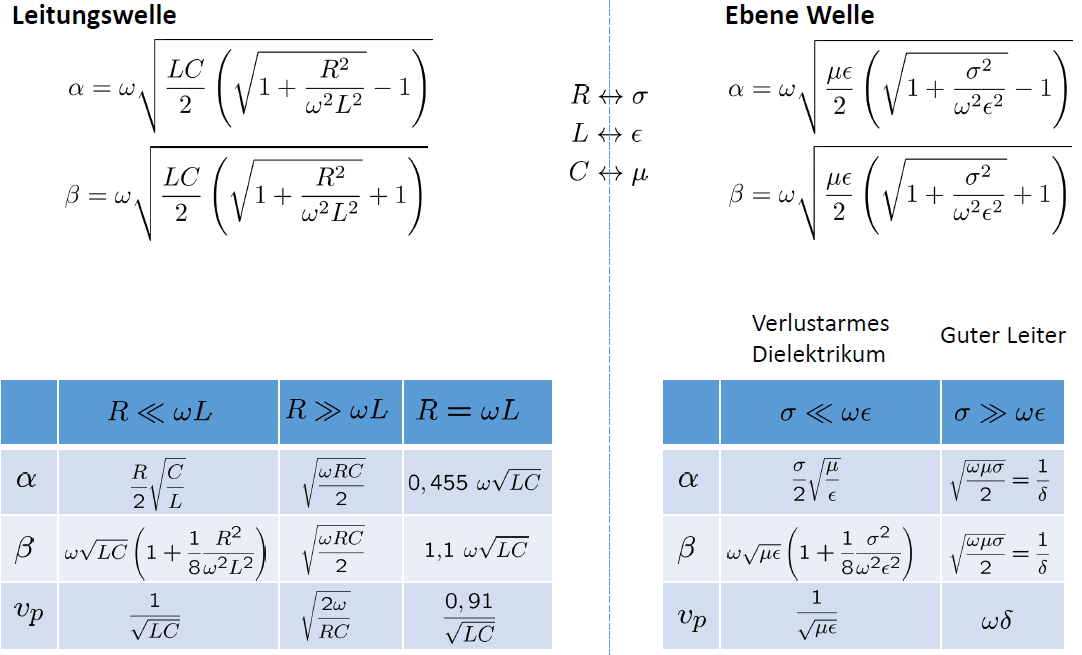
\includegraphics[width=\columnwidth]{Figures/vernachlaessigbarerLeiterwertbelag.png}

\subsection{Übertragungsleitung mit Last}

\def\Hoehe{2};
\def\Breite{8}
\resizebox{0.4\textwidth}{!}{
    %\centering
    \begin{tikzpicture}
        \begin{circuitikz}%[american voltages]
            \draw(0,0)
            to[V,v=$u_G(t)$](0,2)                           %Spannungsquelle
            to[R=$Z_g$](2,2)                               %Quelleninnenwiderstand
            to[short](8,2)
            to[R= $Z_A$](8,0)                               %Lastwiderstand
            to[short](0,0);             
            \draw[-] (2,2) circle (0.1);                    %TOR 1 oben
            \draw[-] (6,2) circle (0.1);                    %TOR 2 oben
            \draw[-] (2,0) circle (0.1);                    %TOR 1 unten
            \draw[-] (6,0) circle (0.1);                    %TOR 2 unten
            \draw[dotted](2,0)--(2,-0.5) node[left]{$l=0$};
            \draw[dotted](2,-0.5)--(2,-1) node[left]{$z=d$};
            \draw[dotted](2,-1)--(2,-1.5);
            \draw[->](2,-0.5) -- (6,-0.5);
            \node at (5,-0,5)[above]{positiv l};

            \draw[dotted](6,0)--(6,-0.5) node[right]{$l=d$};          
            \draw[dotted](6,-0.5)--(6,-1) node[right]{$z=0$};
            \draw[dotted](6,-1)--(6,-1.5);
            \draw[->](6,-1.5) -- (2,-1.5);
            \node at (5,-1,5)[above]{positiv z};

            \draw[->](2,1.25) -- (5,1.25);
            \node at (4,1.25)[above]{forward propagating wave};
            \draw[->](6,0.5) -- (3,0.5);
            \node at (5,0.5)[above]{backward propagating wave};
        \end{circuitikz}
    \end{tikzpicture}
}

\begin{align*}
    U(z) & = U^+ e^{\gamma z} + U^- e^{-\gamma z} = U^+ e^{\gamma d} + U^ - e^{-\gamma d}                      \\
    I(z) & = I^+ e^{\gamma z} + I^- e^{-\gamma z} = \frac{U^+}{Z_L}e^{\gamma d} - \frac{U^-}{Z_L}e^{-\gamma d}
\end{align*}

\subsubsection{Reflexionsfaktor entlang einer Leitung}
\begin{align*}
    r_E    & = r_A  ^{-2\gamma l} = r_A  e^{-2\alpha l} e^{-j2\beta l}                                                     \\
    \alpha & = -\frac{\ln(r_A)}{2l} [\si{Np/m}]                        & \beta & = \dfrac{\phi_2 -\phi_1}{2l} [\si{rad/m}]
\end{align*}

\subsubsection{Stehwellenverhältnis}
\begin{align*}
    \mathrm{SWR} = \frac{U_\text{max}}{U_\text{min}} =
    \frac{I_\text{max}}{I_\text{min}} = \frac{1+|r(z)|}{1-|r(z)|} =
    \frac{|U_H|+|U_R|}{|U_H|-|U_R|}
\end{align*}

\subsubsection{Position von Extrema}
\begin{gather*}
    \boxed{r_A = |r_A|\cdot e^{-j\theta_r}}\rightarrow\theta_r\text{ in rad}\\
    f_\texttt{min}\rightarrow \text{Minimum(Knoten) der Spannungen}\\
    f_\texttt{max}\rightarrow \text{Maximum(Bäuche) der Spannungen}
\end{gather*}
\begin{align*}
    \lambda_\texttt{min/max} & = \frac{c_0}{f_\texttt{min/max}\sqrt{\mu_{r1}\varepsilon_{r1}}}                                                                                                 \\
    z_\texttt{min}           & =\frac{-n\cdot\lambda_\texttt{min}}{2}                                        \qquad\rightarrow n = -\frac{2z}{\lambda_\texttt{min}}                            \\
    z_\texttt{max}           & =\frac{-(2n+1)\lambda_\texttt{max}}{4}                                        \qquad\rightarrow n = -\frac{4z+\lambda_\texttt{max}}{2\cdot\lambda_\texttt{max}} \\
    z                        & = \frac{\lambda_\texttt{min}\cdot\lambda_\texttt{max}}{4(\lambda_\texttt{min}-\lambda_\texttt{max})}
\end{align*}

\subsubsection{Spezialfall: Angepasste Leitung}
\begin{align*}
    Z_A          & = Z_L = Z(z)                              \\
    r_A          & = 0\qquad\rightarrow\text{reflexionsfrei} \\
    \mathrm{SWR} & = 1                                       \\
    U(z)         & = U^+\cdot e ^{j\beta z}                  \\
    I(z)         & = I^+ \cdot e^{j\beta z}                  \\
                 & = \frac{U^+}{Z_L}\cdot e^{j\beta z}
\end{align*}

\subsubsection{Spezialfall: Kurzgeschlossene Leitung}
\begin{align*}
    Z_A          & = 0                                                                        \\
    Z(z)         & = j Z_L\cdot\tan(\beta z)        \qquad\rightarrow\text{rein imaginär}     \\
    r_A          & = -1                                                                       \\
    \mathrm{SWR} & = \infty                                                                   \\
    U(z)         & = U^+\cdot 2j\sin(\beta z)    \qquad\rightarrow U(z=0)=0                   \\
    I(z)         & = U^+\cdot 2\cos(\beta z)    \qquad\rightarrow I(z=0)=I_A=\frac{2U^+}{Z_L}
\end{align*}

\subsubsection{Spezialfall: Leerlaufende Leitung}
\begin{align*}
    Z_A          & = \infty                                                                   \\
    Z(z)         & = -jZ_L\cdot \cot(\beta z) \qquad\rightarrow\text{rein imaginär}           \\
    r_A          & = 1                                                                        \\
    \mathrm{SWR} & = \infty                                                                   \\
    U(z)         & = U^+\cdot 2\cos(\beta z) \qquad\rightarrow U(z=0)=0                       \\
    I(z)         & = U^+\cdot 2j\sin(\beta z) \qquad\rightarrow I(z=0)=I_A = \frac{2U^+}{Z_L}
\end{align*}

\subsubsection{Spezialfall: Ohm'sch abgeschlossene Leitung}
\[
    r_A = \texttt{reell}
\]

\begin{align*}
    \underline{R_A > Z_L} & \rightarrow\theta_r = 0 \rightarrow r_A \texttt{ ist negativ} \\
                          & \rightarrow z_\texttt{max}=\frac{\lambda}{2}\cdot n
\end{align*}

\begin{align*}
    \underline{R_A < Z_L} & \rightarrow\theta_r = \pi                           \\
                          & \rightarrow z_\texttt{min}=\frac{\lambda}{2}\cdot n
\end{align*}

\subsection{Mehrfachreflexionen bei fehlender Anpassung}

\begin{center}
    \begin{tikzpicture}
        %Linien
        \draw[-Latex] (1,1) -- (1,0) node [below] {$t$};
        \draw[-,line width=1pt] (1,1) -- (1,6);
        \draw[-,line width=1pt] (5,0) -- (5,6);

        %Pfeile mit Bezeichnungen
        \draw[-Latex] (3.5,6.5) -- (5,6.5)node[right]{$z$};

        \draw[-Latex] (1,6) -- (5,5) node[right]{$t_D$} node[midway, above]{$U_{1h}$};
        %\draw[-] (1,6) -- (3,5.5) node[above]{$U_{1h}$};

        \draw[-Latex] (5,5) -- (1,4)node[left]{$2t_D$} node[midway, above]{$U_{1r}$};
        %\draw[-] (5,5) -- (3,4.5) node[above]{$U_{1r}$};

        \draw[-Latex] (1,4) -- (5,3)node[right]{$3t_D$} node[midway, above]{$U_{2h}$};
        %\draw[-] (1,4) -- (3,3.5) node[above]{$U_{2h}$};

        \draw[-Latex] (5,3) -- (1,2)node[left]{$4t_D$} node[midway, above]{$U_{2r}$};
        %\draw[-] (5,3) -- (3,2.5) node[above]{$U_{2r}$};

        \draw[-Latex] (1,2) -- (5,1)node[right]{$5t_D$} node[midway, above]{$U_{3h}$};
        %\draw[-] (1,2) -- (3,1.5) node[above]{$U_{3h}$};


        \draw[dotted ] (5,1) -- (3,0.5);

        %Klammern mit Bezeichnungen
        \draw [black,
            decorate,
            decoration = {brace,
                    raise=5pt,
                    amplitude=5pt}] (1,4.2) --  (1,5.8);
        \node at(0.5,5)[left]{$U_{1h}$};

        \draw [black,
            decorate,
            decoration = {brace,
                    raise=5pt,
                    amplitude=5pt}] (5,4.8) --  (5,3.2);
        \node at (5.5,4)[right]{$U_{1h}(1+r_A)$};

        \draw [black,
            decorate,
            decoration = {brace,
                    raise=5pt,
                    amplitude=5pt}] (1,2.2) --  (1,3.8);
        \node at (0.5,3)[left]{$U_{1h}$};
        \node at (0.5,2.5)[left]{$+(1+r_I)U_{1r}$};

        \draw [black,
            decorate,
            decoration = {brace,
                    raise=5pt,
                    amplitude=5pt}] (5,2.8) --  (5,1.2);
        \node at (5.5,2)[right]{$U_{1h}(1+r_A)$};
        \node at (5.5,1.5)[right]{$+U_{2h}(1+r_A)$};


        \draw [black,
            decorate,
            decoration = {brace,
                    raise=5pt,
                    amplitude=5pt}] (1,0.2) --  (1,1.8);
        \node at (0.5,1.5)[left]{$U_{1h}$};
        \node at (0.5,1)[left]{$+(1+r_I)U_{1r}$};
        \node at (0.5,0.5)[left]{$+(1+r_I)U_{2r}$};
    \end{tikzpicture}
\end{center}

\begin{align*}
    %u_{1h} & = u_G\cdot\frac{ Z_L}{R_I + Z_L}            \\
    u_{1r} & = r_A\cdot u_{1h}                                \\
    u_{2h} & = r_I\cdot u_{1r} = r_I\cdot r_A\cdot u_{1h}     \\
    u_{2r} & = r_A\cdot u_{2h} = r_I\cdot r_A^2\cdot u_{1h}   \\
    u_{3h} & = r_I\cdot u_{2r} = r_I^2\cdot r_A^2\cdot u_{1h}
\end{align*}
\resizebox{0.4\textwidth}{!}{
    %\centering
    \begin{tikzpicture}
        \begin{circuitikz}%[american voltages]
            \draw(0,0)
            to[V,v=$u_G(t)$](0,2)   %Spannungsquelle
            to[R=$R_I \neq Z_L$](2,2) %Quelleninnenwiderstand
            to[short](8,2)
            to[R= $R_A\neq Z_L$](8,0)
            to[short](0,0)
            (4,2) to [open, v=$u(z\mathpunct{,}t)$] (4,0) %Spannungspfeil u(z,t)
            (2,2) to [open, v=$u_E(t)$] (2,0) %Spannungspfeil u_E(t)
            (6,2) to [open, v=$u_A(t)$] (6,0); %Spannungspfeil u_A(t)
            \draw[-] (2,2) circle (0.1);
            \draw[-] (6,2) circle (0.1);
            \draw[-] (2,0) circle (0.1);
            \draw[-] (6,0) circle (0.1);
        \end{circuitikz}
    \end{tikzpicture}
}
\begin{align*}
     & \text{Reflexionsfaktor Leitungsanfang: } & \underline{r}_I & = \frac{R_I - Z_L}{R_I + Z_L}                 \\
     & \text{Reflexionsfaktor Leitungsende: }   & \underline{r}_A & = \frac{R_A - Z_L}{R_A + Z_L}                 \\
     & \text{Signallaufzeit: }                  & t_d             & = \frac{l}{c_0}\cdot\sqrt{\mu_r\varepsilon_r} \\
     & \text{Hinlaufende Welle}                 & u_{1h}          & = \hat{u}_G \cdot\frac{Z_L}{Z_L+R_I}
\end{align*}
